% This is samplepaper.tex, a sample chapter demonstrating the
% LLNCS macro package for Springer Computer Science proceedings;
% Version 2.20 of 2017/10/04
%
\documentclass{llncs}
%
\usepackage{graphicx}
% Used for displaying a sample figure. If possible, figure files should
% be included in EPS format.
%
% If you use the hyperref package, please uncomment the following line
% to display URLs in blue roman font according to Springer's eBook style:
% \renewcommand\UrlFont{\color{blue}\rmfamily}

\usepackage{hyperref} % for url
\usepackage{pythonhighlight} % for python

%% listings for python
\usepackage{xcolor}     %高亮使用的颜色
\definecolor{commentcolor}{RGB}{85,139,78}
\definecolor{stringcolor}{RGB}{206,145,108}
\definecolor{keywordcolor}{RGB}{34,34,250}
\definecolor{backcolor}{RGB}{220,220,220}
\usepackage{accsupp}    
\newcommand{\emptyaccsupp}[1]{\BeginAccSupp{ActualText={}}#1\EndAccSupp{}}
\usepackage{listings}
\lstset{                        %高亮代码设置
    language=python,                    %Python语法高亮
    linewidth=0.9\linewidth,            %列表list宽度
    %basicstyle=\ttfamily,              %tt无法显示空格
    commentstyle=\color{commentcolor},  %注释颜色
    keywordstyle=\color{keywordcolor},  %关键词颜色
    stringstyle=\color{stringcolor},    %字符串颜色
    %showspaces=true,                   %显示空格
    numbers=left,                       %行数显示在左侧
    numberstyle=\tiny\emptyaccsupp,     %行数数字格式
    numbersep=5pt,                      %数字间隔
    frame=single,                       %加框
    framerule=0pt,                      %不划线
    escapeinside=@@,                    %逃逸标志
    emptylines=1,                       %
    xleftmargin=3em,                    %list左边距
    backgroundcolor=\color{backcolor},  %列表背景色
    tabsize=4,                          %制表符长度为4个字符
    gobble=4                            %忽略每行代码前4个字符
    }

\begin{document}
%
\title{A Short Instruction for \sf{nnbarrier}}
%
%\titlerunning{Abbreviated paper title}
% If the paper title is too long for the running head, you can set
% an abbreviated paper title here
%
\author{Hengjun Zhao}

\institute{School of Computer and Information Science\\
Southwest University, Chongqing, 400715, P.~R.~China\\
\email{zhaohj2016@swu.edu.cn}}
%
\maketitle % typeset the header of the contribution
%
% \begin{abstract}
% To be completed
% %\keywords{First keyword  \and Second keyword \and Another keyword.}
% \end{abstract}
%
%
\section{Introduction}
In our paper \emph{Synthesizing Barrier Certificates Using Neural Networks} accepted by HSCC'20, we developed a tool named \textsf{nnbarrier}
that can automatically learn a barrier ceritificate represented by a neural network for the safety verification of a continuous dynamical system. 
Here we give a short instruction to the use of \textsf{nnbarrier}, covering the system requirements, installation process, the structure of source codes,
sample inputs, and user-defined inputs. We will emphasize what parts that were presented in the submitted paper will be covered in the instruction, for the purpose of repeatability
evaluation. If there is any problem in using \textsf{nnbarrier}, please contact \email{zhaohj2016@swu.edu.cn}.

\section{Installation}

\subsection{System Requirements}
It is assumed that you have \textsf{Python Version 3.x}  installed on your system.
We have tested \textsf{nnbarrier} on Ubuntu Linux, Mac OS, and Windows (see Table~\ref{tbl:platform}).

\subsection{Dependent Packages}
It is assumed that you have the python package manager \textsf{Pip} installed for \textsf{Python 3.x}, which will facilitate
the installation of dependent packages greatly. 

Essentially, to run \textsf{nnbarrier} without visualization, the only two packages you need to install are \textsf{Pytorch} and \textsf{NumPy}.
It seems that \textsf{numpy} will be automatically installed when installing \textsf{Pytorch}. Please visit \url{https://pytorch.org/} for the 
installation instructions
for the popular machine learning platform \textsf{Pytorch}. For example, with the combination 
\textsf{Mac+Python~3.7+Pip} (without \textsf{cuda} GPU support), the latest stable version \textsf{Pytorch~1.3} can be installed by simply run 
\begin{verbatim}
            pip3 install torch torchvision\end{verbatim}

If you would like to visualize the generated barrier function together with the considered system, i.e. the system dynamics, the domain, the initial set, and the unsafe/safe region,
then some additional graphics packages are required. For visualization of 2D systems, \textsf{matplotlib} needs to be installed, and you are referred to
 \url{https://matplotlib.org/users/installing.html} for the instructions. In the implementation of \textsf{nnbarrier},
 visulaization of 3D systems is supported by \textsf{Mayavi}, a 3D scientific data visualization library. Please visit
 \url{http://docs.enthought.com/mayavi/mayavi/installation.html#installing-with-pip} for the installation of \textsf{mayavi} and 
 its dependencies (e.g. \textsf{PyQt5}). In our testing, on most platforms the visualization-required packages can be installed with the following commands easily:
\begin{verbatim}              
            pip install matplotlib
            pip install mayavi
            pip install PyQt5 \end{verbatim}
where \textsf{pip} can be actually \textsf{pip3}. However, we do met some problems occasionally. If you failed to
get this done in the end, \textsf{nnbarrier} can still be run by commenting the statements for visualization, which
will be explained later.  

In summary, we have tested \textsf{nnbarrier} using the following combinations
\begin{table}
    \centering
	\caption{Tested platforms and packages for \textsf{nnbarrier}}\label{tbl:platform}
	\begin{tabular}{|c|c|c|c|c|c|c|} 
		\hline OS                 & Python    & Pip      & Pytorch & Visualization \\ 
		\hline Ubuntu~18.04.02    & 3.6.7     & 9.0.1    & 1.2.0   & \textsf{matplotlib+mayavi+PyQt5}  \\ 
		\hline Ubuntu~18.04.02    & 3.6.9     & 19.3.1   & 1.3.1   & \textsf{matplotlib+mayavi+PyQt5}  \\ 
        \hline Windows~10~1903    & 3.7.3     & 19.3.1   & 1.3.1   & \textsf{matplotlib+mayavi+PyQt5}  \\
        \hline Mac~OS~10.11.6     & 3.7.6     & 19.3.1   & 1.3.1   & \textsf{matplotlib+mayavi+PySide2}  \\ 
		\hline
	\end{tabular}
\end{table}

\subsection{Obtain the \textsf{nnbarrier} Package}




git clone

\section{Sample Input}

comment some lines


\inputpython{../ann.py}{2}{5}




\begin{python}
    if i==0:
        abc
    else:
        def
\end{python}
python3: --version \pyth{__init__}




\section{Cases in the Paper}

\begin{itemize}
    \item What elements of the paper are included in the REP (e.g.: specific figures, tables, etc.).
    \item Instructions for installing and running the software and extracting the corresponding results. 
\end{itemize}

\section{Define Your Own Problem}

\section{Fine-Tuning}

\subsection{A Subsection Sample}

Please \cite{Prajna04safetyverification} try \cite{BarryICRA2012} avoid rasterized images for line-art diagrams and
schemas. Whenever possible, use vector graphics instead (see
Fig.~\ref{fig1}).

\begin{figure}
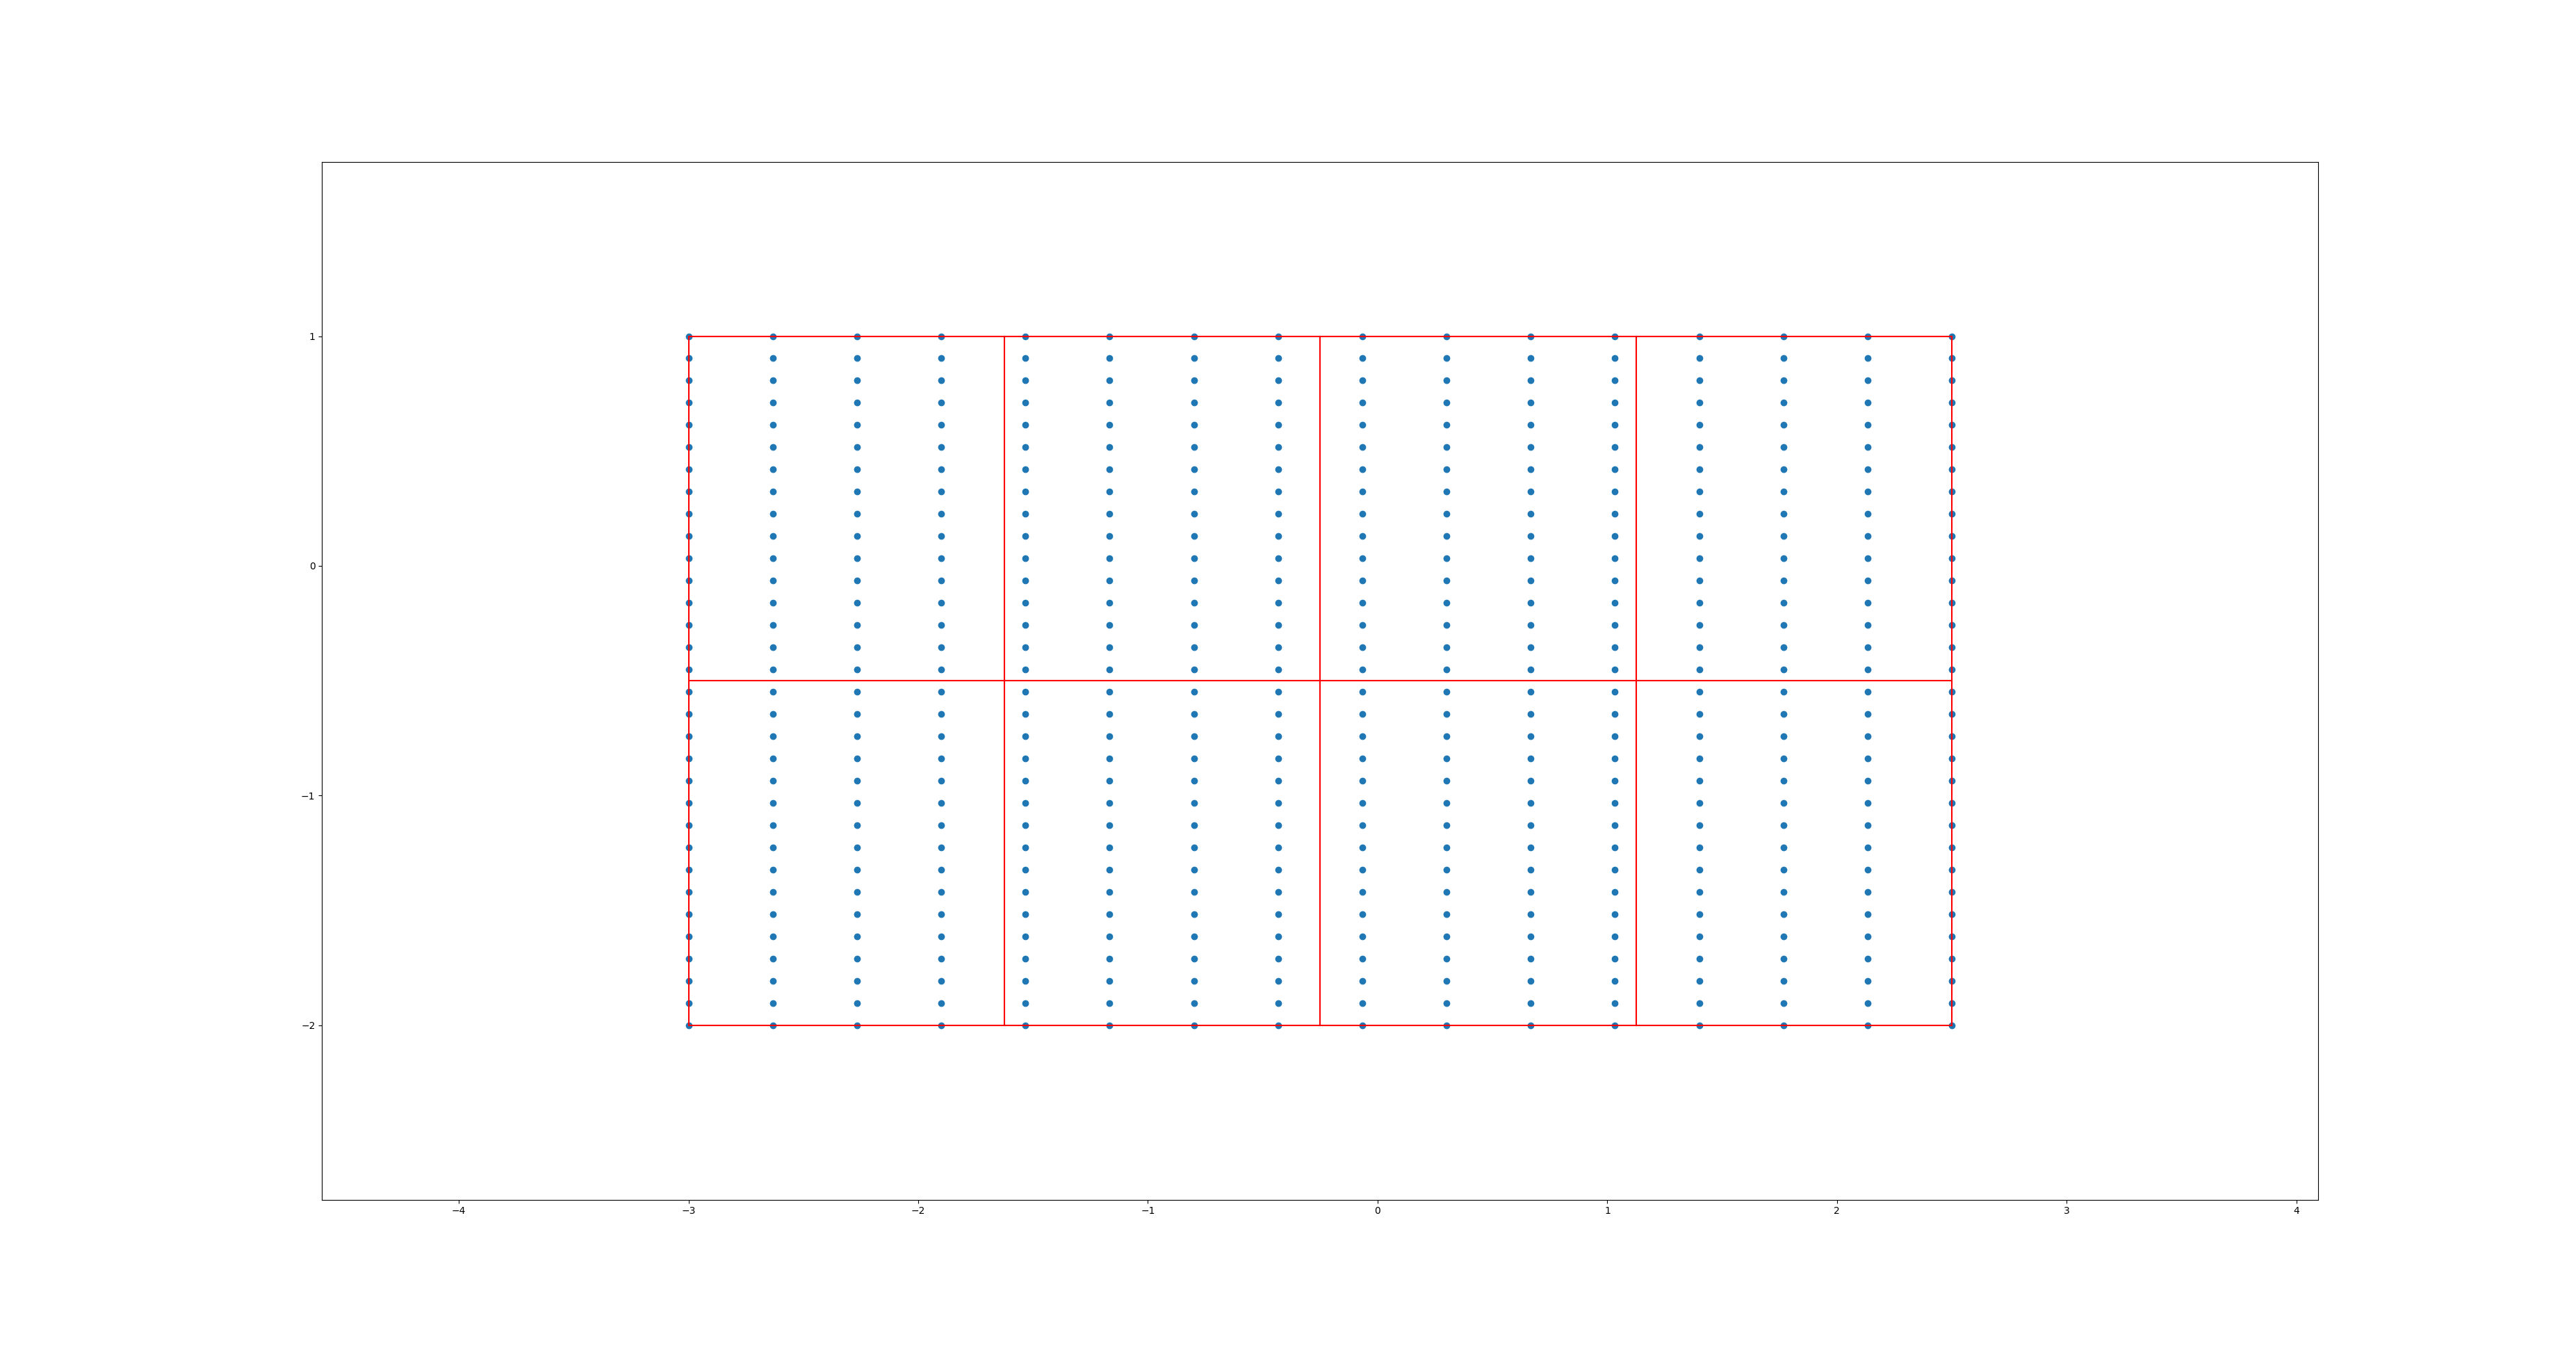
\includegraphics[width=\textwidth]{./fig/batch_data}
\caption{A figure caption is always placed below the illustration.
Please note that short captions are centered, while long ones are
justified by the macro package automatically.} \label{fig1}
\end{figure}

\bibliographystyle{splncs04}
\bibliography{instruction}

% \begin{thebibliography}{8}
% \bibitem{ref_article1}
% Author, F.: Article title. Journal \textbf{2}(5), 99--110 (2016)
% \end{thebibliography}

\end{document}
